\documentclass[a4paper,11pt,twoside]{report}
\usepackage[left=2.5cm,right=2cm,top=2cm,bottom=2cm]{geometry}
\usepackage{ntheorem}
\usepackage{amsmath}
\usepackage{amssymb}
\usepackage{indentfirst}
\usepackage{stmaryrd}
\usepackage{verbatimbox}
\usepackage{amsfonts}
\usepackage{proof}
\usepackage{graphicx}
\usepackage{subfig}
\usepackage{mathtools}
\usepackage{comment}
\newtheorem{def1}{\textbf{Definition}}[chapter]
\newtheorem{exmp}{\textit{Example}}[section]

\begin{document}

\pagenumbering{roman}
\tableofcontents

\relax

\chapter*{Abstract}
\addcontentsline{toc}{chapter}{\numberline{}Abstract}

\chapter*{Acknowledgements}
\addcontentsline{toc}{chapter}{\numberline{}Acknowledgements}
\chapter*{Introduction}
\addcontentsline{toc}{chapter}{\numberline{}Introduction}

\chapter{Lambda Calculus}
\pagenumbering{arabic}
The Lambda Calculus is an example of a formal system which consists a language of lambda terms and some auxiliary notions such as \textit{free variables} and \textit{subterms}, and the transformation theory. The core of the theory is the notion of substitution - the driving force behind function application. 


\section{$\lambda$-terms}

\noindent The expressions in lambda calculus can be formalized into following: 


\begin{def1}
\normalfont \textbf{($\lambda$-TERMS)} $\lambda$-terms can be defined by the following rules:
\end{def1}

\begin{itemize}
\item a variable, $x$, itself is a lambda term
\item if $M$ is a lambda term, and $x$ is a variable, then $(\lambda x.M)$ is a lambda term
\item if $M$ and $N$ are both lambda terms, then \textit{(MN)} is a lambda term
\end{itemize}
A lambda term is valid if and only if it can be obtained by repeated application of these rules. However, some parentheses can be omitted in certain forms. For example the leftmost, outermost brackets are usually omitted.

\textbf{A lambda abstraction $\lambda x.M$} takes a single input x and returns a term M. Thus, it defines an \textbf{anonymous} function. For example $\lambda x.x^2$ is a lambda abstraction for the function $f(x) = x^2$ using the term $x^2$ for M, then we can say that $f = \lambda x.x^2$. The function is anonymous since we write $(x^2)2$ rather than $f3$.

\textbf{An application $(MN)$} applies the input term N to the function M. For example $(\lambda x.x^2)2$ is an application that applies 2 to the function $f(x) = x^2$, it return $2^2$ which equals 4.

As mentioned above, leftmost, outermost brackets are usually omitted. Therefore, $M_1M_2(M_3M_4)$ stands for $((M_1\cdot M_2)(M_3\cdot M_4))$. Similarly, $\lambda$ can be omitted in repeated abstractions, for example $\lambda x_1x_2.M$ stands for $\lambda x_1.(\lambda x_2.M)$.

\begin{def1}
\normalfont (free and bound variables) The set of free and bound variables are defined inductively by the following function:
\end{def1}

\begin{equation*}
\begin{array}{lcllcl}
FV(x)           & = & {x}             & BV(x)           &=& \emptyset\\
FV(\lambda x.M) & = & FV(M_1)\cup {x} & BV(\lambda x.M) &=& FV(M)\backslash y\\  \lambda y.M
FV(MN)          & = & FV(M)\cup FV(N) & BV(MN)          &=& BV(M) \cup BV(N)
\end{array}
\end{equation*}


For example, the lambda term $\lambda x.x$ has no free variables but a bound variable $x$. The function $\lambda x.x+y$ only has a single free variable $y$ and a bound variable $x$. 
Notice that, the sets of bound and free variables are not necessarily disjoint; $x$ occurs both bound and free in:
\begin{equation*}
x(\lambda xy.x)
\end{equation*}

\begin{comment}
\section{Substitution}

\noindent A cursory approach to define the substitution operation leads to the problem of \textit{variable capture}. It occurs when we substitute a term containing a free variable into a scope where the variable becomes bound. For example:
\begin{equation*}
(\lambda xy.xy)y \neq \lambda y.yy
\end{equation*} 

The free occurrence of y in the left hand term becomes confused with the bound variable after substitution.To avoid \textit{variable capture}, we define a capture-avoiding susbstiution. The notion $[x:=N]$ indicates the replacement of a variable $x$ by a term $N$:
\end{comment}
\begin{equation*}
\begin{array}{lrll}
(1)&x[x:=N]&=N & ~\\
(2)&y[x:=N]&=y,& if\ y\neq x\\
(3)&(\lambda y.M)[x:=N]&=\lambda y.M,& if\ y=x\\
(4)&(\lambda y.M)[x:=N]&=\lambda y.(M[x:=N]),& if\ y\notin FV(N)\ \& \ y\neq x\\
(5)&(\lambda y.M)[x:=N]&=\lambda z.(M[y:=z])[x:=N],& if\ y\in FV(N)\ \& \ y\neq x,z\  new\\
(6)&(M_1M_2)[x:=N] &= (M_1[x:=N])(M_2[x:=N])&
\end{array}
\end{equation*}

\begin{def1}\label{def1}
($\alpha$-equivalent) $M$ is $\alpha$-equivalent to $N$, written $M$ $\equiv_\alpha N$, if $N$ results from $M$ by a series of changes of bound variable.
\end{def1}

The notion of alpha-equivalent(or congruence) is a basic form of equivalence defined in lambda calculus. It captures the property that the particular choice of a bound variable in a lambda abstraction does not matter. For instance, $\lambda x.x$ and $\lambda y.y$ are $\alpha$-congruent lambda terms which represent the same function. Notice that, the term-variable $x$ and $y$ are not $\alpha$-equivalent terms since they are not bound in a lambda abstraction.

With the property of alpha equivalence, we can define the \textit{$\alpha$-conversion}:

\begin{equation*}
\lambda x.M =_\alpha \lambda z.(M[z:=x])
\end{equation*}

In some sense, the $\alpha$-conversion is defined by the spirit of the (5) substitution rule. If we have a function $\lambda x.M$, then we can apply a substitution to this function: $(\lambda x.M)[z:=x]$. According to the fifth substitution rule, it is unfolded to $(\lambda z.M[z:=x])$. Using the $\alpha$-conversion, we can always rename the bound variables of a term. 

\begin{def1}
(Variable Convention) If $M_1$,...,$M_n$ occur in a certain context then in these terms all bound variables are chosen to be different from free variables.
\end{def1}

The alpha-conversion is built based on the variable convention. Alpha convertion is used to allow bound variable names to be changed. For example, alpha-conversion of $\lambda x.x$ might get $\lambda y.y$. Terms that differ only by alpha-conversion are called alpha-equivalence(or alpha-congruence) as mentioned in the definition \ref{def1}. By the assumption that free and bound variables are always different(variable convention), and that alpha-conversion will take place whenever a variable is both free and bound. The definition of term substitution becomes:
\begin{equation*}
\begin{array}{rll}
x[x:=N]&=N & ~\\
y[x:=N]&=y,& if\ y\neq x\\
(\lambda y.M)[x:=N]&=\lambda y.(M[x:=N])& \\
(M_1M_2)[x:=N] &= (M_1[x:=N])(M_2[x:=N])&
\end{array} 
\end{equation*}

By this definition of term substitution, the \textit{variable capture} is avoided. Since that y is bound in $\lambda y.M$ of the context:
\begin{equation*}
\lambda y.M[x:=N]
\end{equation*}
y can only be bound in N according to variable convention rule, otherwise, if y is also free in N, it would be renamed by another variable. 

Here is an example of its use:
\begin{equation*}
\begin{array}{ll}
&(\lambda xyz.xzy)(\lambda xz.x)\\
=& \lambda yz.(\lambda xz.x)zy \\
=& \lambda yz.(\lambda xw.x)zy\ \ by\ the\ variable\ convention \\
=& \lambda yz.(\lambda w.z)y\\
=& \lambda yz.z\\
\end{array}
\end{equation*}

\section{$\beta$-reduction}

\noindent There are various notions of reduction for $\lambda$-terms, but the principle one is $\beta$-reduction. $\beta$-reduction is the one-step reduction relation, written as $'\rightarrow _\beta'$. 

\begin{def1}
($\beta$-reduction) For $\lambda$-terms $M$ and $N$, we say that $M$ $\beta$-reduces in one step to $N$, written as $M \rightarrow _\beta N$:
\end{def1}
\begin{equation*}
(\lambda x.M)N\rightarrow _\beta M[x:=N]
\end{equation*}

\begin{equation*}
\frac{M\rightarrow _\beta N}{MZ \rightarrow _\beta NZ}
\end{equation*}
\begin{equation*}
\frac{M\rightarrow _\beta N}{ZM \rightarrow _\beta ZM}
\end{equation*}
\begin{equation*}
\frac{M\rightarrow _\beta N}{\lambda x.M \rightarrow _\beta \lambda x.N}
\end{equation*}

\noindent The reduction relation, written $'\twoheadrightarrow _\beta'$, is the reflexive, transitive closure of the one-step reduction relation. The one-step reduction relation allows a single step of reduction, while the reduction relation allows many steps. The reflexive transitive closure is defined as follows:
\begin{equation*}
\frac{M\rightarrow _\beta N}{M \twoheadrightarrow _\beta N}
\end{equation*}
\begin{equation*}
M \twoheadrightarrow _\beta M
\end{equation*}
\begin{equation*}
\frac{M\twoheadrightarrow _\beta N\ \ \ \ N\twoheadrightarrow _\beta Z}{M \twoheadrightarrow _\beta Z}
\end{equation*}

For the notion $'M\rightarrow _\beta N'$, it is read as '$M$ $\beta$-reduces to $N$'. The first rule defines that the reduction relation is reflexive to one-step reduction relation, while the third rule indicates the transitivity of reduction relation.

\noindent Finally, the $\beta$-equality, written as '$=_\beta$'. For $\lambda$-terms $A$ and $B$, we say that $A =_\beta B$ if either $A \equiv B$ or there exists a sequence of reduction starting with $A$, ending with $B$. It is the equivalence relation generated by $\twoheadrightarrow _\beta$:

\begin{equation*}
\frac{M\twoheadrightarrow _\beta N}{M = _\beta N}
\end{equation*}
\begin{equation*}
\frac{M = _\beta N}{N = _\beta M}
\end{equation*}
\begin{equation*}
\frac{M = _\beta N\ \ \ \ N = _\beta Z}{M = _\beta Z}
\end{equation*}

For the notion $'M = _\beta N'$, we say '$M$ $\beta$-equivalent to $N$'. 

\noindent Following is a simple example which applies $\beta$-reduction:

\begin{equation*}
\begin{array}{ll}
&(\lambda x.x^2)3\\
=& (x^2)[x:=3] \\
=& 3^2 \\
=&9 \\
\end{array}
\end{equation*}


\begin{def1}
($\beta$-redex) A $\beta$-redex of a $\lambda$-term $M$ is a subterm of M of the form ($\lambda$x.P)Q. A term M is called in $\beta$-normal form if it has no $\beta$-redex.
\end{def1}
A $\beta$-redex is essentially a candidate for an application of $\beta$-reduction. A term $M$ has a $\beta$-normal form if there exists a term N such that N is in $\beta$-normal form and $M \twoheadrightarrow _\beta N$. 

\section{Head Normal Form}

\noindent A $\lambda$-term in head normal form is generally in the form:

\begin{equation*}
\lambda x_1\ldots x_n.xM_1\ldots M_m\ \ \ \ \ \ \ \ n,m\geqslant 0
\end{equation*}

In this case $x$ is called the head variable. If $M \equiv \lambda x_1\ldots x_n.(\lambda x.M_0)M_1\ldots M_m$ where $n\geqslant 0$, $m\geqslant 1$ then the subterm $(\lambda x.M_0)M_1$ is called the head redex of $M$. Following are some examples of $\lambda$-terms in head normal form:
\begin{equation*}
(1)\ xM\ \ \ \ (2)\ \lambda x.x\ \ \ \ (3)\ \lambda xy.x((\lambda z.z)y)
\end{equation*}Normal order:
Notice that, an expression in head normal form may contain redexes in argument positions whereas a normal form may not.


\section{Reduction strategies}\label{sec:reductionstrategy}
\noindent Recall that a term is said to be in $\beta$-normal form if it has no $\beta$-redexes, that is, subterms of the shape ($\lambda$x.M)N. A term has a $\beta$-normal form if it can be reduced to a term in $\beta$ in $\beta$-normal form. It is clear that if a term has a $\beta$-normal form, then we can get to the $\beta$-normal form by exhaustively reducing all $\beta$-redexes of the term, then reducing all $\beta$-redexes of all resulting terms, and so forth until we get the $\beta$-normal form. A \textbf{$\beta$-reduction strategy} is a function that selects, whenever a term has multiple $\beta$-redexes, which one should be reduced first. If a term is in $\beta$-normal form, then no $\beta$-reduction is to be done. Notice that, a $\beta$-reduction strategy may or may not have the property that adhering to the strategy will ensure that we(eventually) reach a $\beta$-normal form, if one exists. 

In general, there are several different $\beta$-reductions possible for a given term. In this project, there are 5 different reduction strategies studied and implemented: normal order, call-by-name, call-by-value, head reduction, and applicative order. Figure X generally summarizes and compares the property of different strategies:
 
\begin{center}
\begin{table}[ht!]
\begin{tabular}{|c|c|c|c|}\hline
Reduction Strategy & Reduction Order & Reach $\beta$-normal form & Form Reached\\ \hline
Normal Order & leftmost outermost & Yes & normal form\\ \hline
Call-by-name & leftmost outermost & No  & weak head normal form\\ \hline
Call-by-value & leftmost innermost & No & weak normal form\\ \hline
Head Reduction & inside lambda abstractions & No & head normal form\\ \hline
Applicative Order & leftmost innermost & Yes & normal form\\ \hline
\end{tabular}
\caption{Reduction Strategies}
\end{table}
\end{center}
Normal order:
We model lambda terms as Haskell constructed data, representing variable names by character:

\begin{verbatim}
type Name = Char  

data Term = Var Name | Abs Name Term | App Term Term
            deriving (Show, Eq)
\end{verbatim}


\subsection*{Operational Semantics}

A sequence of computational steps of a valid program is the operational semantics for the programming language. The final step of a terminating sequence returns the resulting value of the program. Operational semantics can be classified into two types: \textbf{structural operational semantics(SOS or small-step semantics)} and \textbf{natural semantics(NS or big-step semantics)}. The structural operational semantics describes each single step of a computation in a program, while the natural semantics describes the overall resulting value generated by the program. Following, we use both SOS and NS to define the behavior of each reduction strategy. The small-step semantics gives reduction rules of the strategy, when the big-step semantics describes how the final term is reached.  

\subsection*{Recursion}

Although a reduction strategy may or may not have the property that ensures it reaches a $\beta$-normal form, it would recursively contract the selected redex until no redex(decided by specific reduction strategy) can be contracted. All the following Haskell functions defined conrresponding to the reduction strategy model the small-step semantics. Therefore, in order to recursively reduce a $\lambda$-term, an auxiliary function \verb|recur_eval :: Term -> IO()| is defined:

\begin{verbatim}
       recur_eval :: Term -> IO()
       recur_eval t | evalcbn t == t = putStrLn("")
                    | otherwise = do
                                putStrLn("==> "++ tostring (evalcbn t))
                                recur_eval (evalcbn t)
\end{verbatim}

The Haskell function above defines the recursive reduction by Call-by-Name strategy. It uses the small-step function defined in Section \ref{subsec:cbn}. The recursion will terminate if the input $\lambda$-term cannot be reduced anymore, otherwise, it would print-out the term after a single step reduction and continue reducing the resulting term.



\subsection{Normal Order Reduction}{\label{subsec:normal}}

The normal order reduction $e\xrightarrow{no} e'$ continually applies te rule for $\beta$-reduction on the redex in leftmost outermost position until no more $\beta$-reduction can be performed. At that point, the resulting term is in normal form. When reducing an application $(e_1e_2)$, the function term $e_1$ must be reduced using call-by-name. Since the strategy is outermost, when $e_1$ is reduced to an abstraction $(\lambda x.e)$, then the redex $((\lambda x.e)e_2)$ must be reduced before redexes in e.

\begin{equation*}
\llceil x \rrfloor ^{ls} _{no} = x
\end{equation*}
\begin{equation*}
\frac{\llceil e \rrfloor ^{ls} _{no} = e'}{\llceil (\lambda x.e) \rrfloor ^{ls} _{no} = (\lambda x.e')}
\end{equation*}
\begin{equation*}
\frac{\llceil e_1 \rrfloor ^{ls} _{cbn} = (\lambda x.e)\ \ \ \ \ \ \ \ \ \llceil e[e_2/x] \rrfloor ^{ls} _{no} = e'}{\llceil (e_1e_2) \rrfloor ^{ls} _{no} = e'}
\end{equation*}
\begin{equation*}
\frac{\llceil e_1 \rrfloor ^{ls} _{cbn} = e'_1\neq (\lambda x.e)\ \ \ \ \ \ \ \ \llceil e'_1 \rrfloor ^{ls} _{no} = e''_1\ \ \ \ \ \ \ \ \llceil e_2 \rrfloor ^{ls} _{no} = e'_2}{\llceil (e_1e_2) \rrfloor ^{ls} _{no} = (e''_1e'_2)}
\end{equation*}

\begin{center}
Normal Order: Big-step operational semantics
\end{center}

\begin{equation*}
\frac{}{(\lambda x.M)N \rightarrow _\beta M[N/x]}\ \  
\frac{M \rightarrow _\beta N}{MP \rightarrow _\beta NP}\ \ 
\frac{M \rightarrow _\beta N}{PM \rightarrow _\beta PN}(P\ \textit{contains no redex})\ \ 
\frac{M \rightarrow _\beta N}{(\lambda x.M) \rightarrow _\beta (\lambda x.N)}
\end{equation*}
\begin{center}
Normal Order: Small-step operational semantics
\end{center}

Normal order reduction is \textit{normalizing}, since it reduces the $\lambda$-term until there is no redex, redex in abstractions is also contracted. So, the normal order reduction will terminate with the normal form as result. 

The corresponding Haskell function \verb|evalnormal :: Term -> Term| below implements the normal order reduction. Notice that, it uses the function evalcbn defined in \ref{subsec:cbn}:

\begin{verbatim}
       evalnormal :: Term -> Term
       evalnormal (Var x) = Var x
       evalnormal (Abs x t) = (Abs x (evalnormal t))
       evalnormal (App (Abs x t) v) = subs t (Var x, v)
       evalnormal (App x t) | x == evalcbn x = (App x (evalnormal t))
                            | otherwise = (App (evalcbn x) t)
\end{verbatim}

The first function clause above handles variables $x$. It is not a $\beta$-reduction step, since a variable is not a redex. It returns itself which indicates no reduction can be done. It also conforms the pattern matching mechanism in Haskell. Similarly, the second function clause handles abstractions $(\lambda x.e)$ and implements the fourth SOS rule. The third function handles applications $(e_1e_2)$ when $e_1$ is an abstraction, then the substitution will take place. It applies an argument to the function and returns the resulting value. Finally, the fourth function handles  applications $(e_1e_2)$ when $e_1$ is not an abstraction. Since the normal reduction is leftmost outermost, it reduces the function $e_1$ first. If $e_1$ cannot be reduced(returns itself), then it goes to the argument $e_2$. 


Folllowing is the running example of normal order reduction in Haskell. We use ``/'' to represent the $\lambda$ symbol:

\begin{verbatim}
           (/a.a)(/b.b)((/x.x)(/y.(/z.z)w))
       ==> (/b.b)((/x.x)(/y.(/z.z)w))
       ==> (/x.x)(/y.(/z.z)w)
       ==> /y.(/z.z)w
       ==> /y.w
       Reduced to:/y.w
\end{verbatim}


As we can see, it uses leftmost outermost strategy. The leftmost outermost redex $(\lambda a.a)(\lambda b.b)$ is first reduced. Then the whole reduced term is a redex, the argument $((\lambda x.x)(\lambda y.(\lambda z.z)w))$ substitutes the bound variables in the abstraction $(\lambda b.b)$. After that, the same substitution take place. Finally, it reaches into the redex $(\lambda z.z)w$ in the abstraction $\lambda y.(\lambda z.z)w$ and generates the resulting term $\lambda y.w$


\subsection{Call-by-Name Reduction}{\label{subsec:cbn}}

The Call-by-Name reduction $e\xrightarrow{cbn} e'$ reduces the leftmost outermost redex not insde a lambda abstraction first. That is, the arguments to a function are not evaluated before the function is called. The redex in $e$ of the asbtraction $(\lambda x.e)$ will never be reduced. 


\begin{equation*}
\llceil x \rrfloor ^{ls} _{cbn} = x
\end{equation*}
\begin{equation*}
\llceil (\lambda x.e) \rrfloor ^{ls} _{cbn} = (\lambda x.e)
\end{equation*}
\begin{equation*}
\frac{\llceil e_1 \rrfloor ^{ls} _{cbn} = (\lambda x.e)\ \ \ \ \ \ \ \ \ \llceil e[e_2/x] \rrfloor ^{ls} _{cbn} = e'}{\llceil (e_1e_2) \rrfloor ^{ls} _{cbn} = e'}
\end{equation*}
\begin{equation*}
\frac{\llceil e_1 \rrfloor ^{ls} _{cbn} = e'_1\neq (\lambda x.e)}{\llceil (e_1e_2) \rrfloor ^{ls} _{cbn} = (e'_1e_2)}
\end{equation*}
\begin{center}
Call-by-Name: Big-step operational semantics
\end{center}

\begin{equation*}
\frac{}{(\lambda x.M)N \rightarrow _\beta M[N/x]}\ \ \ \  
\frac{M \rightarrow _\beta N}{MP \rightarrow _\beta NP}\ \ 
\end{equation*}
\begin{center}
Call-by-Name: Small-step operational semantics
\end{center}

The Call-by-Name reduction generates term in weak head normal form. A lambda expression is in weak head normal form if it is a head normal form or any lambda abstraction. 


The corresponding Haskell function \verb|evalcbn :: Term -> Term| below implements the Call-by-Name reduction:

\begin{verbatim}
       evalcbn :: Term -> Term
       evalcbn (Var x) = Var x
       evalcbn (Abs x t) = (Abs x t)
       evalcbn (App (Abs x t) y) = subs t (Var x, y)
       evalcbn (App x y) | x == evalcbn x = (App x y)
	                     | otherwise = (App (evalcbn x) y) 
\end{verbatim}


The first two function clauses handle the variables and abstractions, it returns itself since they cannot be reduced under Call-by-Name reduction. The third function implements the first SOS rule which performs substitution. The last function implements the second SOS rule: if the function $e_1$ of the application $(e_1e_2)$ cannot be reduced, then the argument $e_2$ will never be reduced. 

The same example in \ref{subsec:normal} run in Haskell by the Call-by-Name strategy is as follows:

\begin{verbatim}
           (/a.a)(/b.b)((/x.x)(/y.(/z.z)w))
       ==> (/b.b)((/x.x)(/y.(/z.z)w))
       ==> (/x.x)(/y.(/z.z)w)
       ==> /y.(/z.z)w
       Reduced to:/y.(/z.z)w
\end{verbatim}

It is easy to see that the first three reduction steps are the same as normal order reduction. In this example, it stops at $\lambda y.(\lambda z.z)w$. Since the only difference between normal order and call-by-name is the redex inside abstractions will never be reduced in call-by-name. 


\subsection{Call-by-Value Reduction}{\label{subsec:cbv}}

Call-by-Value reduction is the most common reduction strategy. In Call-by-Value, the argument expression is evaluated, and the resulting value is bound to the corresponding variable in the function. It first reduces the leftmost innermost redex not inside an abstraction. It never reduces a redex when the argument is not a \textit{value}. It differs from Call-by-Name only by reducing the argument $e_2$ of the application $(e_1e_2)$ before the substitution take place. 


\begin{equation*}
\llceil x \rrfloor ^{ls} _{cbv} = x
\end{equation*}
\begin{equation*}
\llceil (\lambda x.e) \rrfloor ^{ls} _{cbn} = (\lambda x.e)
\end{equation*}
\begin{equation*}
\frac{\llceil e_1 \rrfloor ^{ls} _{cbv} = (\lambda x.e)\ \ \ \ \ \ \ \ \ \llceil e_2 \rrfloor ^{ls} _{cbv} = e'_2\ \ \ \ \ \ \ \ \ \ \llceil e[e'_2/x] \rrfloor ^{ls} _{cbv}  = e'}{\llceil (e_1e_2) \rrfloor ^{ls} _{cbv} = e'}
\end{equation*}
\begin{equation*}
\frac{\llceil e_1 \rrfloor ^{ls} _{cbv} = e'_1\neq (\lambda x.e)\ \ \ \ \ \ \ \ \ \llceil e_2 \rrfloor ^{ls} _{cbv} = e'_2}{\llceil (e_1e_2) \rrfloor ^{ls} _{cbv} = (e'_1e'_2)}
\end{equation*}
\begin{center}
Call-by-Value: Big-step operational semantics
\end{center}

\begin{equation*}
\frac{}{(\lambda x.M)N \rightarrow _\beta M[N/x]}\ \ \ \  
\frac{M \rightarrow _\beta N}{MP \rightarrow _\beta NP}(M\ \textit{not an abstraction})\ \ \ \
\frac{M \rightarrow _\beta N}{VM \rightarrow _\beta VN}(M\ \textit{not an abstraction})\ \ \ 
\end{equation*}
\begin{center}
Call-by-Value: Small-step operational semantics
\end{center}

Call-by-Value generates terms in weak head normal form only. The implementation of the rules by an Haskell function \verb|evalcbv :: Term -> Term| is as follows:

\begin{verbatim}
        evalcbv :: Term -> Term
        evalcbv (Var x) = Var x
        evalcbv (Abs x t) = (Abs x t)
        evalcbv (App (Abs x t) y) = subs t (Var x, evalcbv y)
        evalcbv (App x y) | x == evalcbn x = (App x (evalcbv y))
                          | otherwise = (App (evalcbn x) y)  
\end{verbatim}

The functions are similar to Call-by-Name, the only difference is the argument is reduced before the substitution take place as indicated in the function clause 3.

The sample example run in Haskell by the Call-by-Value strategy is as follows:

\begin{verbatim}
            (/a.a)(/b.b)((/x.x)(/y.(/z.z)w))
        ==> (/b.b)((/x.x)(/y.(/z.z)w))
        ==> (/b.b)(/y.(/z.z)w)
        ==> /y.(/z.z)w
        Reduced to:/y.(/z.z)w
\end{verbatim}

As we can see, the reduction procedure is different from previous. It differs from previous two strategies at the second reduction step. Since the call-by-value reduction always reduces the argument before the substitution take place, it reduces the redex in the argument $((\lambda x.x)(\lambda y.(\lambda z.z)w))$ before it replaces the bound variables in the function $(\lambda b.b)$.    


\subsection{Head Reduction}

The head reduction performs reductions inside lambda abstractions, but only in head position. Notice that, the \textit{head reduction} strategy introduced in this project is the same as defined by Barendregt \cite{barendregt1984lambda}, however it differs from Sessoft's \cite{sestoft2002demonstrating} \textit{head spine reduction}. In the leftmost head reduction, only head redexes are reduced. A redex $((\lambda x.e_0)e_1)$ is a \textit{head redex} if it is proceded to the left only by lambda abstractions of non-redexes, as in $\lambda x_1...\lambda x_n.(\lambda x.e_0)e_1...e_m$ when $n \geqslant 0\ and\ m \geqslant 1$.


\begin{equation*}
\llceil x \rrfloor ^{ls} _{hr} = x
\end{equation*}
\begin{equation*}
\frac{\llceil e \rrfloor ^{ls} _{hr} = e'}{\llceil (\lambda x.e) \rrfloor ^{ls} _{hr} = (\lambda x.e')}
\end{equation*}
\begin{equation*}
\frac{\llceil e_1 \rrfloor ^{ls} _{cbn} = (\lambda x.e)\ \ \ \ \ \ \ \ \ \llceil e[e_2/x] \rrfloor ^{ls} _{hr} = e'}{\llceil (e_1e_2) \rrfloor ^{ls} _{hr} = e'}
\end{equation*}
\begin{equation*}
\frac{\llceil e_1 \rrfloor ^{ls} _{cbn} = e'_1\neq (\lambda x.e)}{\llceil (e_1e_2) \rrfloor ^{ls} _{hr}  = (e'_1e_2)}
\end{equation*}
\begin{center}
Head Reduction: Big-step operational semantics
\end{center}


\begin{equation*}
\frac{}{(\lambda x.M)N \rightarrow _\beta M[N/x]}\ \ \ \ \  
\frac{M \rightarrow _\beta N}{MP \rightarrow _\beta NP}\ \ \ \ \ 
\frac{M \rightarrow _\beta N}{(\lambda x.M) \rightarrow _\beta (\lambda x.N)}
\end{equation*}
\begin{center}
Head Reduction: Small-step operational semantics
\end{center}

The head reduction strategy generates terms in head normal form. Recall that, a term is in head normal form if it has the form: $\lambda x_1\ldots x_n.xM_1\ldots M_m\ \ \ \ n,m\geqslant 0$

\begin{verbatim}
       headreduction :: Term -> Term
       headreduction (Var x) = Var x
       headreduction (Abs x t) = (Abs x (headreduction t))
       headreduction (App (Abs x t) y) = subs t (Var x, y)
       headreduction (App x y) | x == evalcbn x = (App x y)
                               | otherwise = (App (evalcbn x) y)  
\end{verbatim}

The first 3 function clauses are similar as before, it transfers the semantic rules straght forward into Haskell functions. The last function clause uses Call-by-Name function defined in \ref{subsec:cbn}, because it has to avoid premature reduction of inner redexes. 


The sample example run by Head Reduction is as follows:

\begin{verbatim}
         (/a.a)(/b.b)((/x.x)(/y.(/z.z)w))
     ==> (/b.b)((/x.x)(/y.(/z.z)w))
     ==> (/x.x)(/y.(/z.z)w)
     ==> /y.(/z.z)w
     ==> /y.w
     Reduced to:/y.w
\end{verbatim}

The reduction procedure is the same as normal order reduction. Notice that, in the third reduction step, the redex $(\lambda z.z)w$ is a head redex in the abstraction $\lambda y.(\lambda z.z)w$. 

\subsection{Applicative Order Reduction}

Applicative order reduction $e\xrightarrow{ao} e'$ reduces the leftmost innermost redex first. A function's arguments are always reduced before the function itself. Applicative order always attempts to apply functions to normal forms. It differs from Call-by-Value only by reducing also under abstractions:


\begin{equation*}
\llceil x \rrfloor ^{ls} _{ao} = x
\end{equation*}
\begin{equation*}
\frac{\llceil e \rrfloor ^{ls} _{ao} = e'}{\llceil (\lambda x.e) \rrfloor ^{ls} _{ao} = (\lambda x.e')}
\end{equation*}
\begin{equation*}
\frac{\llceil e_1 \rrfloor ^{ls} _{ao} = (\lambda x.e)\ \ \ \ \ \ \ \ \ \llceil e_2 \rrfloor ^{ls} _{ao} = e'_2\ \ \ \ \ \ \ \ \ \ \llceil e[e'_2/x] \rrfloor ^{ls} _{ao} = e'}{\llceil (e_1e_2) \rrfloor ^{ls} _{ao} = e'}
\end{equation*}
\begin{equation*}
\frac{\llceil e_1 \rrfloor ^{ls} _{ao} = e'_1\neq (\lambda x.e)\ \ \ \ \ \ \ \ \ \llceil e_2 \rrfloor ^{ls} _{ao} = e'_2}{\llceil (e_1e_2) \rrfloor ^{ls} _{ao} = (e'_1e'_2)}
\end{equation*}
\begin{center}
Applicative Order: Big-step operational semantics
\end{center}

\begin{equation*}
\frac{}{(\lambda x.M)N \rightarrow _\beta M[N/x]}(\textit{M, N in normal form})\ \ \ \ 
\frac{M \rightarrow _\beta N}{MP \rightarrow _\beta NP}\ \ \ \ 
\frac{M \rightarrow _\beta N}{PM \rightarrow _\beta PN}(P\ \textit{contains no redex})\ \ \ \ 
\end{equation*}
\begin{equation*}
\frac{M \rightarrow _\beta N}{(\lambda x.M) \rightarrow _\beta (\lambda x.N)}
\end{equation*}
\begin{center}
Applicative Order: Small-step operational semantics
\end{center}

Applicative orde reduction always generates terms in normal form. Since it also reduce the redexes in abstractions. The applicative order reduction is not normalizing, functions applied to non-normalizing arguments are non-normalizing.



\begin{verbatim}
      apporder :: Term -> Term
      apporder (Var x) = Var x
      apporder (Abs x t) = (Abs x (apporder t))
      apporder (App (Abs x t) y) = subs t (Var x, y)
      apporder (App x y) | x == apporder x = (App x (apporder y))
                         | otherwise = (App (apporder x) y)  
\end{verbatim}

The function clauses are simliar to the Call-by-Value introduced in \ref{subsec:cbv}. The only difference is the redexex inside abstractions are also reduced.


The sample example run by Applicative Order reduction in Haskell is as follows:

\begin{verbatim}
             (/a.a)(/b.b)((/x.x)(/y.(/z.z)w))
         ==> (/b.b)((/x.x)(/y.(/z.z)w))
         ==> (/x.x)(/y.(/z.z)w)
         ==> /y.(/z.z)w
         ==> /y.w
         Reduced to:/y.w
\end{verbatim}

It is the same as normal order reduction and the resulting term $\lambda y.w$ is in normal form. Although applicative order reduction always reduces the leftmost innermost redex, there is no redex on leftmost has an inner redex. If we make the leftmost abstraction $(\lambda a.a)$ become $(\lambda a.(\lambda c.c)w)$, then the first reduction step would reduce the inner redex $(\lambda c.c)w$ first:

\begin{verbatim}
             (/a.(/c.c)w)(/b.b)((/x.x)(/y.(/z.z)w))
         ==> (/a.w)(/b.b)((/x.x)(/y.(/z.z)w))
         ==> (/b.b)((/x.x)(/y.(/z.z)w))
         ==> (/x.x)(/y.(/z.z)w)
         ==> /y.(/z.z)w
         ==> /y.w
         Reduced to:/y.w
\end{verbatim}


\section{Comparisons between Different Reduction Strategies }








\chapter{The Curry type assignment system}

A type system consists a set of rules that assign a property called a \textit{type} to the various constructs --- such as variable, expression, functions or modules. There are several reasons to add types to a program, one of the most important reason to add type properties to a program is to reduce bugs. It is possible to build an abstract interpretation of programs by treating terms as objects. The abstractions can be regarded as the interface of objects, by checking whether the interfaces have been connected properly we can decide whether the program is defined in a consistent way. Moreover, type systems provide a form of documentation and improve the readability of a program. Since a program can be abstracted, there are less information in the structure of a program. Furthermore, it also enables independent compilation before the implementation of a program runs. The types of functions and arguments can be checked during the generation of codes. Type-checking during implementation enables dynamic  debugging which largely reduces the debugging workload at run-time. If a program is error-free, it is safe to run:"Typed programs cannot go wrong". It also allows multiple dispatch which is the feature of some objected-oriented programming languages in which a function or method can be dynamically dispatched based on the run time type of more than one of its arguments.
 
An exmaple of a type system is the Java language. A Java program consists of classes which contains a set of function definitions. A function is invoked by an instance of a class that the function belongs to. The interface of a function states the type of the return value, the name of the function and a list of values that are passed to the function. The code of an invoking function states the object instance on which this particular method is to be invoked, and the name of this function along with the names of variables that hold values to pass to it. The Java compiler checks the type of each argument that passed into the function, against the type declared for each varaible in the interface of the invoked function. If the types do not match, the compiler throws a compile-time error.

The lambda calculus as treated in Chapter 1 is referred to as a \textit{type-free} theory. Because every expression may be applied to every other expression. For example, the $\lambda x.x$ may be applied to any argument $x$ and generates the same $x$. 

The typed version of lambda calculus(or called Combinatory Logic, a variant of the lambda calculus) is introduced essentially in Curry\ref{curry1934functionality} and in Church(1940). Types are objects of a syntactic nature and may be assigned to lambda terms. If M is a lambda term and a type A is assigned to M, then we say \textit{`M has type A'}; the notation used is $`M:A'$. For example, in a typed system one has $\lambda x.x : (A \rightarrow A)$, which means the function $\lambda x.x$ should take an argument in type $A$ and return a value of type $A$. In general, $A \rightarrow B$ is the type of functions from $A$ to $B$.

\section{The System $\lambda \rightarrow $-Curry}

In Curry and Feys(1958) and Curry et al. the type assignment theory was modified in a natural way to the lambda calculus assigning elements of a given set $\mathbb{T}$ of types to type free lambda terms. For this reason these calculi are sometimes called systems of type assignment. If the type $\sigma \in \mathbb{T}$ is assigned to the term $M \in \Lambda$ which writes as $\vdash M : \sigma$, sometime with a under subcript such as $\vdash _\lambda$ to denote the particular system. Usually a set of assumptions $\Gamma$ is needed to derive a type assignment write as $\Gamma \vdash M : \sigma$(read as `$\Gamma$ yields $M$ in $\sigma$').

\begin{def1}
\normalfont (i) The set of $types$, notation $\mathbb{T}$, 
\end{def1} 

Notation. (i) If $\sigma _1,...,\sigma _n \in \mathbb{T}$ then

\begin{equation*}
\sigma _1 \rightarrow \sigma _2 \rightarrow ... \rightarrow \sigma _n
\end{equation*}

\noindent stands for
\begin{equation*}
(\sigma _1 \rightarrow (\sigma _2 \rightarrow ... \rightarrow (\sigma _{n-1} \rightarrow \sigma _n)))
\end{equation*}

\noindent we use association to the right.

     (ii) $\alpha,\beta,\gamma,...$ denote arbitrary type variables.


\begin{def1}
\normalfont (i) A \textit{statement} is of the form $M : \sigma$, where $M\in \Lambda$ and $\sigma \in \mathbb{T}$(pronounced as $`M\ in\ \sigma'$). $M$ is called the $subject$ and $A$ the $predicate$ of $M : A$.  
\end{def1}
(ii) A $context$ $\Gamma$ is a set of statements with only distinct (term) variables as subjects; In \cite{svb2001type}, the notion $\Gamma,M:\sigma$ is used for the context $\Gamma \cup \{M:\sigma\}$ where either $M:\sigma \in \Gamma$ or $M$ does not occur in $\Gamma$, and we use $M:\sigma$ as shorthand for $\emptyset,M:\sigma$.


\begin{def1}
\normalfont (CF. [\ref{curry1934functionality}, \ref{curry1972combinatory}]) Curry type assignment and $derivations$ can be defined using following derivation rules.  
\end{def1}

\begin{equation*}
(1):\frac{}{\Gamma ,M:\sigma \vdash _cM:\sigma} 
\end{equation*}
\begin{equation*}
(2):\frac{\Gamma ,x:\sigma \vdash _cM:\beta}{\Gamma \vdash _c(\lambda x.M):\sigma \rightarrow \beta} 
\end{equation*}
\begin{equation*}
(3):\frac{\Gamma \vdash _cM_1:\sigma \rightarrow \beta\ \ \ \ \ \Gamma \vdash _cM_2:\sigma}{\Gamma \vdash _c(M_1M_2):\beta} 
\end{equation*}

\begin{exmp}
\normalfont (i)Let $\sigma \in \mathbb{T}$. Then $\Gamma \vdash \lambda fx.f(fx):(\sigma \rightarrow \sigma)\rightarrow \sigma \rightarrow \sigma$, is shown by the following derivation:
\end{exmp}

$$
\infer[(2)]{\Gamma \vdash \lambda fx.f(fx):(\sigma \rightarrow \sigma)\rightarrow \sigma \rightarrow \sigma}{
	\infer[(1)]{\Gamma \vdash \lambda x.f(fx):\sigma \rightarrow \sigma}{
      \infer{\Gamma \vdash f(fx):\sigma}{
             \infer[(1)]{\Gamma,f:\sigma \rightarrow \sigma \vdash f:\sigma \rightarrow \sigma}{}
             & 
             \infer{\Gamma \vdash fx:\sigma}{
                \infer{\Gamma,f:\sigma \rightarrow \sigma \vdash f:\sigma \rightarrow \sigma}{}
                &
                \infer{\Gamma,x:\sigma \vdash x:\sigma}{}
             }
         }
      }		
	}
$$


(ii)Notice that, we cannot type \textit{`self-application'} $xx$. In order to type the application $xx$, the derivation should be as following:

$$
\infer{\Gamma \vdash xx:B}{
    \infer{\Gamma \vdash x:A \rightarrow B}{} 
    &
    \infer{\Gamma \vdash x:A}{}
}
$$


As we can see, the term variable $x$ is assigned to two types: $A \rightarrow B$ and $A$, and either of them can be substituted by the other one. So, $A \rightarrow B \neq A$, and there are two statements of subject $x$ in context $\Gamma$ with distinct predicates. Those two statements would be conflict according to the definition of context. Therefore, the `self-application' is untypable. 



\section{Subject Reduction}

\section{Properties of $\lambda \rightarrow $}

\begin{def1}
\normalfont (Type substitution(van Bakel\ref{svb2001type})) The substitution $(\varphi \mapsto C): $, where $\varphi$ is a type variable and $C \in \mathbb{T}$ is defined as following:
\end{def1}

\begin{equation*}
\begin{array}{ll}
(\varphi \mapsto C)\varphi        & = C\\
(\varphi \mapsto C)\varphi '      & = \varphi ',if\ \varphi '\neq \varphi\\
(\varphi \mapsto C)A\rightarrow B & = ((\varphi \mapsto C)A)\rightarrow ((\varphi \mapsto C)B)
\end{array}
\end{equation*}


\begin{def1}
\normalfont Let $Id_s$ be the substitution that replaces all type variables by themselves:
\end{def1}

\noindent (i) Robinson's unification algorithm. Unification of Curry types is defined by:

\begin{equation*}
\begin{array}{llll}
unify & \varphi            & \varphi          & = (\varphi \mapsto \varphi)\\
unify & \varphi            & B                & = (\varphi \mapsto B), if\ \varphi does\ not\ occur\ in\ B\\
unify & A                  & \varphi          & = unify\ \ \varphi\ \ A\\
unify & (A\rightarrow B)   & (C\rightarrow D) & = S_1\circ S_2\\
&&&\ \ \ where\ S_1 = unify\ \ A\ \ C\\
&&&\ \ \ \ \ \ \ \ \ \ \ \ S_2 = unify\ (S_1B)\ (S_1D)
\end{array}
\end{equation*}


\noindent (ii) UnifyContexts

\begin{equation*}
\begin{array}{llll}
UnifyContexts & (\Gamma _0,x:A) & (\Gamma _1,x:B) & = S_1\circ S_2\\
&&&\ \ \ where\ S_1 = unify\ \ A\ \ B\\
&&&\ \ \ \ \ \ \ \ \ \ \ \ S_2 = UnifyContexts\ (S_1\Gamma _0)\ (S_1\Gamma _1)\\
UnifyContexts & (\Gamma _0,x:A) & \Gamma _1 & = UnifyContexts\ \Gamma _0\ \Gamma _1, if\ x\ does\ not\ occur\ in\ \Gamma _1\\
UnifyContexts & \varnothing & \Gamma _1 & =  Id_s
\end{array}
\end{equation*}



\begin{def1}
\normalfont (PPC, Principle Pair Algorithm for $\Lambda$)
\end{def1}

\begin{equation*}
\begin{array}{llll}
ppc & x & = & \langle x:\varphi,\varphi \rangle\\
&&& where\ \ \varphi=fresh\\
ppc & (\lambda x.M) & = & \langle \Pi,A \rightarrow P \rangle,\ if\ ppcM=\langle \Pi \cup \{x:A\},P \rangle\\
&&& \langle \Pi,\varphi \rightarrow P \rangle,\ if\ ppcM=\langle \Pi ,P \rangle\ \ \ \ x\not\in \Pi\\
&&&\ \ \ \ \ \ \ \ \ \ \ \ \ \ \ \ \ where\ \varphi=fresh\\
ppc & (MN) & = & S_1\circ S_2\langle \Pi _1\cup \Pi _2,\varphi \rangle\\
&&& where\ \ \ \varphi \ \ \ \ \ \ \ \ \ \ \ = fresh\\
&&& \ \ \ \ \ \ \ \ \ \ \langle \Pi _1,P_1,\varphi \rangle = ppcM\\
&&& \ \ \ \ \ \ \ \ \ \ \langle \Pi _2,P_2,\varphi \rangle = ppcN\\
&&& \ \ \ \ \ \ \ \ \ \ S_1 \ \ \ \ \ \ \ \ \ \ \ = unify\ P_1\ \ (P_2 \rightarrow \varphi)\\
&&& \ \ \ \ \ \ \ \ \ \ S_2 \ \ \ \ \ \ \ \ \ \ \ = UnifyContexts\ (S_1\Pi _1)\ (S_1\Pi _2)\\
\end{array}
\end{equation*}


\chapter{A Purely-Functional Programming Language --- Haskell}

\section{Functional Programming}
\section{Haskell}
\section{Model the $\lambda$-calculus and the Curry Type Assignment System in Haskell}
\section{Issues and Weakness of Implementation in Haskell }



\chapter{The $\lambda$-calculus and Curry Type Assignment System Implementation in Java}
The Java version of implementation is transferred directly from Haskell. However, the semantics and operational order of Haskell is difference from Java, especially the `where' statement of Haskell. The 'where' declaration is called when the defined variables are used, however, in Java, we need to separate a `where' block into parts according to where it is called. An example is shown in Section \ref{sec:hj}. This differece is worth taking care of when transfer the Haskell into Java, otherwise, NullPointerException may occur. 

In all data types, the method toString() has been implemented -- more precisely overridden, as it is a method of the Java primary class\verb| Object|. This function is used to print out the data type as a string. There are more method signatures defined in the interfaces as a reference to instantiable classes. 

\section{Different operational order between Haskell and Java}{\label{sec:hj}}
As mentioned above, the operaional order of Haskell is different from Java, not only the pattern matching, but also the `where' declarations. Since the code in Haskell cannot be transferred into Java directly, it largely abandoned the simplicity of codes. Following is a piece of code that defines principle pair algorithm:
\begin{verbatim}
ppc :: Term -> [Char] -> (PPc, [Char])
ppc (Abs x y) r | contains (Var x) pi = ((removeItem (Var x, a) pi, (TP a p)), tl1)
                | otherwise = ((pi, (TP f p)), tl1)
                            where (f, tl) = fresh r                    (1) 
                                  ((pi, p), tl1) = ppc y tl            (2)
                                  (_, a) = search (Var x) pi           (3)

\end{verbatim}

`Guards' are used as an if-then-else block. There are three declarations in the `where' block each with a distinct number. For the first condition of ppc function, declaration (1)(2)(3) are called since all the declared variables are used. In the `otherwise' condition, only declaration (1)(2) are called. In this case, in order to transfer the Haskell function into Java methods, we need to repetitively define the variables which largely reduces the simplicity of codes. 





\begin{verbatim}
public PPC ppc(Term term, String counter){
     ...
     else if(term instanceof Abstraction){
        Variable xv = new Variable(((Abstraction) term).getName());
        PPC receiver = ppc(((Abstraction) term).getTerm(), counter);
        if(receiver != null){
           if(contains(xv, receiver.getSubject())){
             Type searchType = search(xv, receiver.getSubject()).getPredicate();
             ArrayList<Statement> original = receiver.getSubject().getContext();
             ArrayList<Statement> remove = new ArrayList<>();

             for(Statement s: original){
               if(s.getSubject().equals(xv)) remove.add(s);
             }

             for(Statement rm: remove){
                original.remove(rm);
             }

             TP tp = new TP(searchType, receiver.getPredicate());
             return new PPC(new Context(original), tp, receiver.getCounter());
          }
          else{
             TVar f = new TVar(receiver.getCounter().substring(0, 1));
             return new PPC(receiver.getSubject(), new TP(f, receiver.getPredicate()),
                            receiver.getCounter().substring(1));

          }
       }
       else {
           return null;
       }
     }
     ...
}
\end{verbatim}

\section{$\lambda$-calculus Representation}
\subsection{$\lambda$-terms}
A Lambda term can either be a variable, an abstraction or an application. An interface `Term' is defined as a reference type, which has three lambda term implementations. This is the generic representation of all lambda terms.

\begin{figure}[ht]
\centering
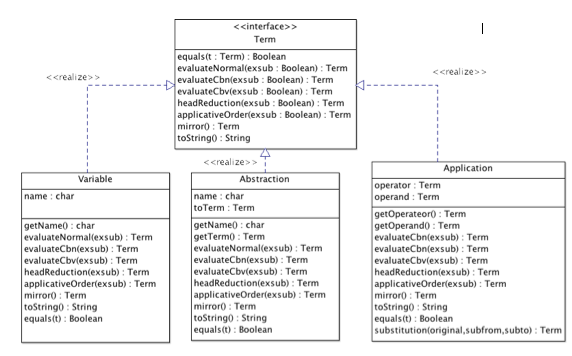
\includegraphics[scale=0.7]{Term}
\caption{Class diagram of Lambda Calculus data structures}
\label{fig:term1}
\end{figure}

This interface defines the method \verb|equals(Term t)|, which return a boolean states whether it is equal to the input term. This method overrides the \verb|equals(Object o)| method of the Java primary class \verb|Object|. It is essential in the reduction procedure, since we can decide whether a term is reducible by compare the term before reduction and after. If the term is the same as it before reduction, then it cannot be reduced. Therefore, we know when we can stop the reduction procedure.  

As mentioned in Section \ref{sec:reductionstrategy}, there are five reduction strategies enabled in the reducer. So there are five method signatures defined in the interface: \textsf{evaluateNormal(Bool exsub), evaluateCbn(Bool exsub), evaluateCbv(Bool exsub), headReduction(Bool exsub), applicativeOrder(Bool exsub)}. Each of these method refers to a specific reduction strategy as the method name. 

The method \textsf{mirror()} is used to create a mirror term with exactly the same class variables. This method is used when the substitution is performed. For example, if we have a lambda term $\lambda f.(\lambda x.f(xx))(\lambda x.f(xx))$, it is reduced to $\lambda f.f((\lambda x.f(xx))(\lambda x.f(xx)))$. If we do not create a mirror term of $(\lambda x.f(xx))$, both of these two $(\lambda x.f(xx))$ would refer to the same memory space. In other words, the abstraction $(\lambda x.f(xx))$ is used twice to form an application. Therefore, if operations performed on the function, it is also performed on the argument. It is essential to create a mirror term that separate those two terms although they look exactly the same.      

Finally, the \textsf{toString()} method of class \textsf{Object} is overridden to transform a lambda term to a string. 

Notice that, in the implementation class \verb|Application|, there is a \textsf{substitution(Term original, Term subfrom, Term subto):Term} method. It is used to substitute bound variables in an abstraction, which is an application function, to the argument. The first parameter of the method is the body of abstraction, the second argument states which bound variable could be substituted and the third argument states what it could be substituted to.

\subsection{Interpreter}
To allow interactions and inputs from users, the program needs to interpret the input term into a data structure in the system. Figure \ref{fig:inter} illustrates all the methods that used to interpret an input into a lambda term data structure.   

\begin{figure}[ht]
\centering
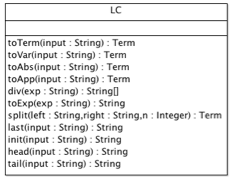
\includegraphics[scale=0.6]{LC}
\caption{Interpretation methods in LC class}
\label{fig:inter}
\end{figure}

The method \textsf{toTerm(String input)} takes a string as input and returns a \textsf{Term}. It calls \textsf{toVar(String input), toAbs(String input)} or \textsf{toApp(String input)} according to type of the outermost term. Then, those three methods iteratively call each other until the whole term is interpreted.   

\textsf{div(String exp)} divides an application into the function and argument. Basically, it return an array with 2 string elements. The method \textsf{toExp(String exp)} is used to remove brackets of applications and returns an expression that is bracker-free. Finally, the most important method \textsf{split(String left, String right, Int n)} implements the bracket removal mechanism. It marks the right most right bracker `)' and find the matching left bracket `(' and extract the term out without brackets.

Since the Java implementation is directly transferred from Haskell, there are also four basic string operations which are Haskell builit-in functions. \textsf{last(String input)} takes a string and returns the last character of the string, it returns itself if the length of input string is 1. \textsf{init(String input)} accepts a string and returns the string without its last character, it returns an empty string if it only contains one character. \textsf{head(String input)} takes a string and returns the first element of the string, it returns itself when the input string length is 1. \textsf{tail(String input)} takes a string and returns the string without its first element, it returns an empty string when the length of input is 1. 

Following is the example of how those Haskell built-in function work:

\begin{verbatim}
              init "Hello"   "Hell"            head "Haskell"   "H" 
              init "A"       ""                head "A"         "A"
\end{verbatim}

\begin{verbatim}
              last "String"   "g"              tail "Lambda"   "ambda" 
              last "A"        "A"              tail "A"         ""
\end{verbatim}


\section{Curry Type Assignment System Representation}



\begin{figure}[ht]
\centering
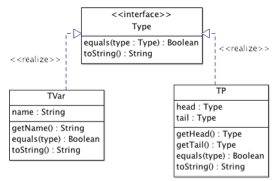
\includegraphics[scale=0.7]{Type}
\caption{type}
\label{fig:type}
\end{figure}


\begin{figure}[ht]
\centering
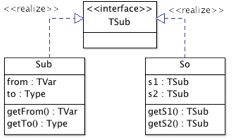
\includegraphics[scale=0.7]{TSub}
\caption{Class diagram of Lambda Calculus data structures}
\label{fig:term1}
\end{figure}


\begin{figure}[ht]
\centering
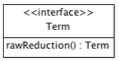
\includegraphics[scale=0.7]{TermRaw}
\caption{Class diagram of Lambda Calculus data structures}
\label{fig:term1}
\end{figure}


\begin{figure}
\centering
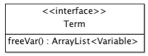
\includegraphics[scale=0.7]{TermType}
\caption{Class diagram of Lambda Calculus data structures}
\label{fig:term1}
\end{figure}



\begin{figure}
\centering
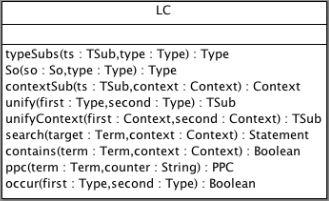
\includegraphics[scale=0.6]{LCType}
\caption{Class diagram of Lambda Calculus data structures}
\label{fig:term1}
\end{figure}


\begin{figure}
\centering
\begin{minipage}{.3\textwidth}
\centering
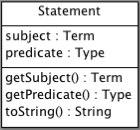
\includegraphics[scale=0.8]{Statement}
\caption{Caption for figure 1}
\label{fig:test1}
\end{minipage}\hfill
\begin{minipage}{.3\textwidth}
\centering
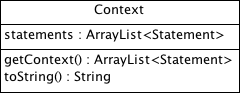
\includegraphics[scale=0.65]{Context}
\caption{Caption for figure 2}
\label{fig:test2}
\end{minipage}\hfill
\begin{minipage}{.3\textwidth}
\centering
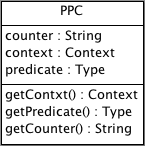
\includegraphics[scale=0.7]{PPC}
\caption{Caption for figure 3}
\label{fig:test3}
\end{minipage}
\end{figure}


\section{Auxiliary Functions}

\section{Syntax and Interpreter}

\chapter{GUI development}

\section{Layout}

\section{Functionalities}

\chapter{Java vs Haskell, Pros and Cons}

\section{Pros}

\section{Cons}

\chapter{Conclusion}


\bibliographystyle{plain}
\bibliography{ref}

\end{document}